%%%%%%%%%%%%%%%%%%%%%%%%%%%%%%%%%%%%%%%%%%%%%%%%%%%%%%%%%%%%%%%%%%%%%%%%%%%%%%%
\subsection{Introduction and Motivations}
%%%%%%%%%%%%%%%%%%%%%%%%%%%%%%%%%%%%%%%%%%%%%%%%%%%%%%%%%%%%%%%%%%%%%%%%%%%%%%%
\begin{frame}
 \begin{colorblock}{blue}{lightblue}{ }
    \Large \textbf{Introduction and Motivations}
  \end{colorblock}
\end{frame}

\begin{frame}
\frametitle{Hadoop 1.0: Focus on Batch applications}
\begin{figure}[h]
  \centering
  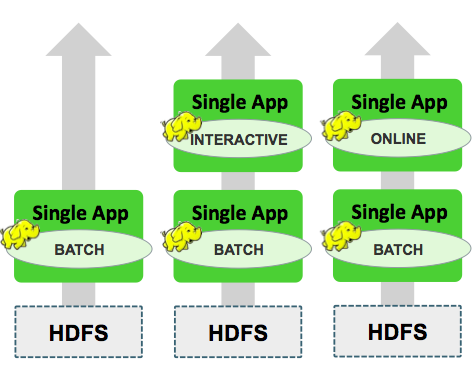
\includegraphics[scale=0.4]{./figures/yarn_hadoop1}
  \label{fig:yarn_h1}
\end{figure}
\begin{itemize}
	\item {\bf Built for batch applications}
	\begin{itemize}
		\item Supports only MapReduce applications
	\end{itemize}
	\item {\bf Different silos for each usage pattern}
\end{itemize}
\end{frame}

\begin{frame}
\frametitle{Hadoop 1.0: Architecture (reloaded)}
\begin{columns}[onlytextwidth]
  \begin{column}{0.3\textwidth}
    \begin{figure}[h]
    \centering
    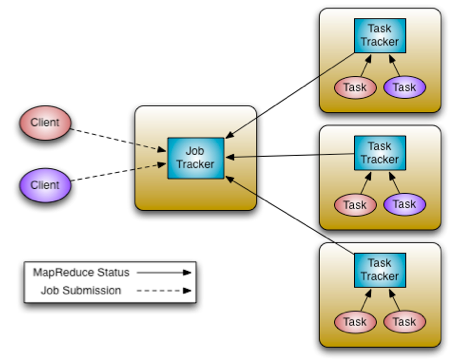
\includegraphics[scale=0.35]{./figures/yarn_hadoop1_arch}
    \label{fig:yarn_h1_arch}
    \end{figure}
  \end{column}

  \begin{column}{0.5\textwidth}
    \begin{itemize}
      \item {\bf JobTracker}
      \begin{itemize}
        \item Manages cluster resources
        \item Performs Job scheduling
        \item Performs Task scheduling
      \end{itemize}

\vspace{20pt}

      \item {\bf TaskTracker}
      \begin{itemize}
        \item Per machine agent
        \item Manages Task execution
      \end{itemize}
    \end{itemize}
  \end{column}
\end{columns}
\end{frame}

\begin{frame}
\frametitle{Hadoop 1.0: Limitations}
\begin{itemize}
  \item {\bf Only supports MapReduce, no other paradigms}
  \begin{itemize}
    \item Everything needs to be cast to MapReduce
    \item Iterative applications are slow
  \end{itemize}

\vspace{10pt}

  \item {\bf Scalability issues}
  \begin{itemize}
    \item Max cluster size roughy 4,000 nodes
    \item Max concurrent tasks, roughly 40,000 tasks
  \end{itemize}

\vspace{10pt}

  \item {\bf Availability}
  \begin{itemize}
    \item System failures destroy running and queued jobs
  \end{itemize}

\vspace{10pt}

  \item {\bf Resource utilization}
  \begin{itemize}
    \item Hard, static partitioning of resources in Map or Reduce slots
    \item Non-optimal resource utilization
  \end{itemize}
\end{itemize}
\end{frame}

\begin{frame}
\frametitle{Next Generation Hadoop}
\begin{figure}[h]
  \centering
  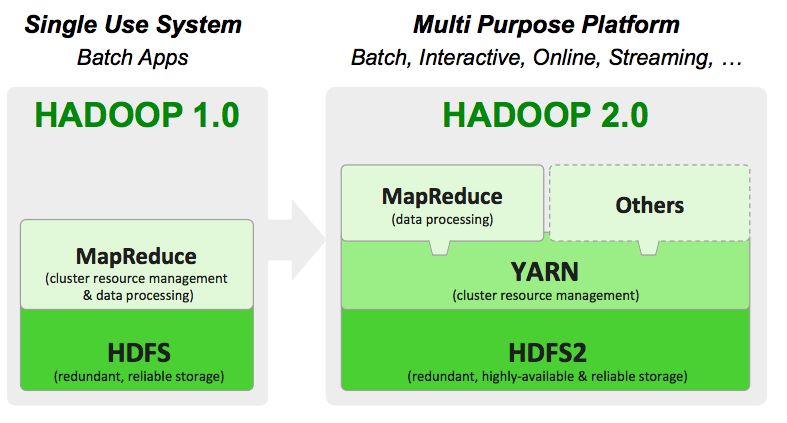
\includegraphics[scale=0.4]{./figures/yarn_vision}
  \label{fig:yarn_vision}
\end{figure}
\end{frame}

\begin{frame}
\frametitle{The YARN ecosystem}
\begin{figure}[h]
  \centering
  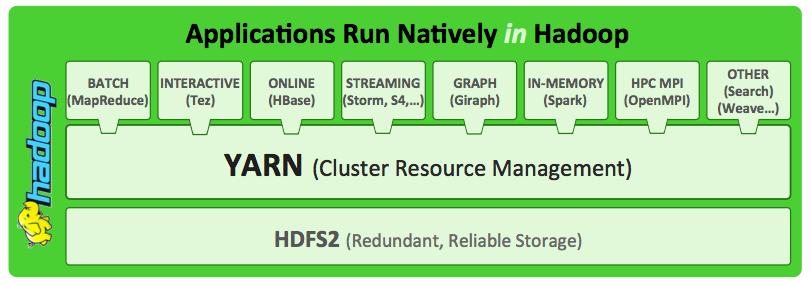
\includegraphics[scale=0.4]{./figures/yarn_ecosystem}
  \label{fig:yarn_ecosystem}
\end{figure}
\begin{itemize}
  \item {\bf Store all data in one place}
  \begin{itemize}
    \item Avoids costly duplication
  \end{itemize}
  \item {\bf Interact with data in multiple ways}
  \begin{itemize}
    \item Not only in batch mode, with the rigid MapReduce model
  \end{itemize}
  \item {\bf More predictable performance}
  \begin{itemize}
    \item Advanced scheduling mechanisms
  \end{itemize}
\end{itemize}
\end{frame}

\begin{frame}
\frametitle{Key Improvements in YARN (1)}
\begin{itemize}
  \item {\bf Support for multiple applications}
  \begin{itemize}
    \item Separate generic resource brokering from application logic
    \item Define protocols/libraries and provide a framework for custom application development
    \item Share same Hadoop Cluster across applications
  \end{itemize}

\vspace{10pt}

  \item {\bf Improved cluster utilization}
  \begin{itemize}
    \item Generic resource container model replaces fixed Map/Reduce slots
    \item Container allocations based on locality and memory
    \item Sharing cluster among multiple application
  \end{itemize}

\vspace{10pt}

  \item {\bf Improved scalability}
  \begin{itemize}
    \item Remove complex app logic from resource management
    \item State machine, message passing based loosely coupled design
    \item Compact scheduling protocol
  \end{itemize}
\end{itemize}
\end{frame}

\begin{frame}
\frametitle{Key Improvements in YARN (2)}
\begin{itemize}
  \item {\bf Application Agility}
  \begin{itemize}
    \item Use Protocol Buffers for RPC gives wire compatibility
    \item Map Reduce becomes an application in user space
    \item Multiple versions of an app can co-exist leading to experimentation
    \item Easier upgrade of framework and applications
  \end{itemize}

\vspace{20pt}

  \item {\bf A data operating system: shared services}
  \begin{itemize}
    \item Common services included in a pluggable framework
    \item Distributed file sharing service
    \item Remote data read service
    \item Log Aggregation Service
  \end{itemize}
\end{itemize}
\end{frame}

%%%%%%%%%%%%%%%%%%%%%%%%%%%%%%%%%%%%%%%%%%%%%%%%%%%%%%%%%%%%%%%%%%%%%%%%%%%%%%%
\subsection{YARN Architecture Overview}
%%%%%%%%%%%%%%%%%%%%%%%%%%%%%%%%%%%%%%%%%%%%%%%%%%%%%%%%%%%%%%%%%%%%%%%%%%%%%%%
\begin{frame}
 \begin{colorblock}{blue}{lightblue}{ }
    \Large \textbf{YARN Architecture Overview}
  \end{colorblock}
\end{frame}

\begin{frame}
\frametitle{YARN: Architecture Overview}
\begin{figure}[h]
  \centering
  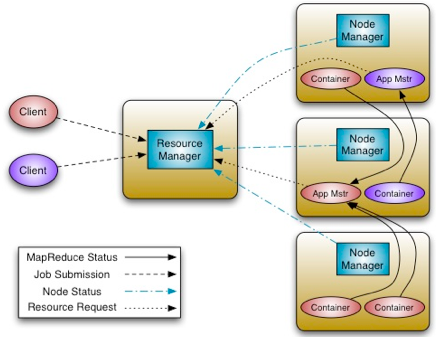
\includegraphics[scale=0.5]{./figures/yarn_arch}
  \label{fig:yarn_arch}
\end{figure}
\end{frame}

\begin{frame}
\frametitle{YARN: Design Decisions}
\begin{itemize}
  \item {\bf No static resource partitioning}
  \begin{itemize}
    \item There are no more slots
    \item Nodes have resources, which are allocated to applications when requested
  \end{itemize}
  \item {\bf Separate resource management from application logic}
  \begin{itemize}
    \item Cluster-wide resource allocation and management
    \item Per-application master component
    \item Multiple applications $\to$ multiple masters
  \end{itemize}
\end{itemize}
\begin{figure}[h]
  \centering
  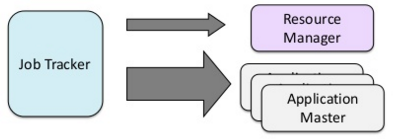
\includegraphics[scale=0.5]{./figures/yarn_key_idea}
  \label{fig:yarn_key_idea}
\end{figure}
\end{frame}

\begin{frame}
\frametitle{YARN Daemons}
\begin{itemize}
  \item {\bf Resource Manager (RM)}
  \begin{itemize}
    \item Runs on master node
    \item Global resource manager and scheduler
    \item Arbitrates system resources between {\bf competing} applications
  \end{itemize}
  \item {\bf Node Manager (NM)}
  \begin{itemize}
    \item Run on slave nodes
    \item Communicates with RM
    \item Reports utilization
  \end{itemize}
  \item {\bf Resource containers}
  \begin{itemize}
    \item Created by the RM upon request
    \item Allocate a certain amount of resources on slave nodes
    \item Applications run in one or more containers
  \end{itemize}
  \item {\bf Application Master (AM)}
  \begin{itemize}
    \item One per application, {\bf application specific}\footnote{Every new application requires a new AM to be designed and implemented!}
    \item Requests more containers to execute application tasks
    \item Runs in a container
  \end{itemize}
\end{itemize}
\end{frame}

\begin{frame}
\frametitle{YARN: Example with 2 Applications}
\begin{figure}[h]
  \centering
  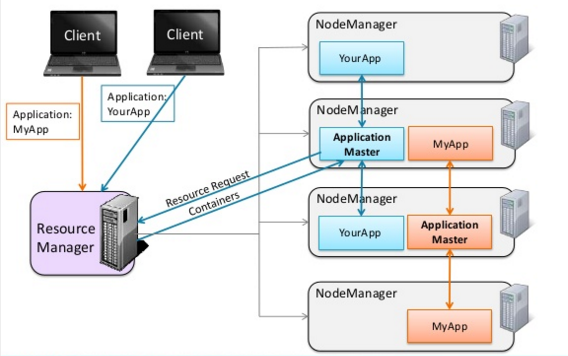
\includegraphics[scale=0.4]{./figures/yarn_ex1}
  \label{fig:yarn_ex1}
\end{figure}
\end{frame}

%%%%%%%%%%%%%%%%%%%%%%%%%%%%%%%%%%%%%%%%%%%%%%%%%%%%%%%%%%%%%%%%%%%%%%%%%%%%%%%
\subsection{YARN Core Components}
%%%%%%%%%%%%%%%%%%%%%%%%%%%%%%%%%%%%%%%%%%%%%%%%%%%%%%%%%%%%%%%%%%%%%%%%%%%%%%%
\begin{frame}
 \begin{colorblock}{blue}{lightblue}{ }
    \Large \textbf{YARN Core Components}
  \end{colorblock}
\end{frame}

\begin{frame}
\frametitle{YARN Schedulers (1)}
\begin{itemize}
  \item {\bf Schedulers are a pluggable component of the RM}
  \begin{itemize}
    \item In addition to existing ones, advanced scheduling is supported
  \end{itemize}

\vspace{20pt}

  \item {\bf Current supported schedulers}
  \begin{itemize}
    \item The Capacity scheduler
    \item The Fair scheduler
    \item Dominant Resource Fairness
  \end{itemize}

\vspace{20pt}

  \item {\bf What's different w.r.t. Hadoop 1.0?}
  \begin{itemize}
    \item Support any YARN application, not just MapReduce
    \item No more slots, tasks are scheduled based on resources
    \item Some terminology change
  \end{itemize}
\end{itemize}
\end{frame}

\begin{frame}
\frametitle{YARN Schedulers (2)}
\begin{columns}[onlytextwidth]
  \begin{column}{0.3\textwidth}
    \begin{figure}[h]
    \centering
    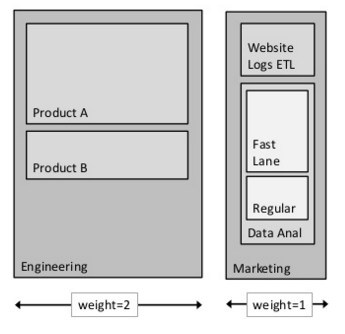
\includegraphics[scale=0.45]{./figures/yarn_queues}
    \label{fig:yarn_queues}
    \end{figure}
  \end{column}

  \begin{column}{0.5\textwidth}
    \begin{itemize}
      \item {\bf Hierarchical queues}
      \begin{itemize}
        \item Queues can contain sub-queues
        \item Sub-queues share resources assigned to queues
      \end{itemize}
    \end{itemize}
  \end{column}
\end{columns}
\end{frame}

\begin{frame}
\frametitle{YARN Resource Manager: Overview}
  \begin{figure}[h]
    \centering
    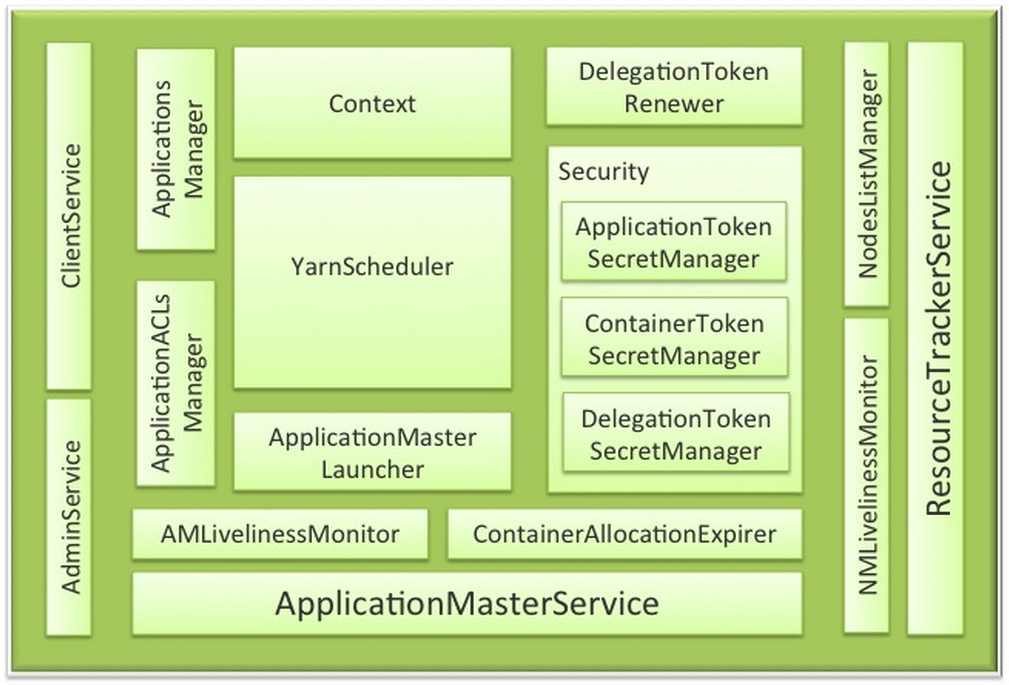
\includegraphics[scale=0.25]{./figures/yarn_RM}
    \label{fig:yarn_RM}
  \end{figure}
\end{frame}

\begin{frame}
\frametitle{YARN Resource Manager: Operations}
\begin{itemize}
  \item {\bf Node Management}
  \begin{itemize}
    \item Tracks hearbeats from NMs
  \end{itemize}

\vspace{20pt}

  \item {\bf Container Management}
  \begin{itemize}
    \item Handles AM requests for new containers
    \item De-allocates containers when they expire or application finishes
  \end{itemize}

\vspace{20pt}

  \item {\bf AM Management}
  \begin{itemize}
    \item Creates a container for every new AM, and tracks its health
  \end{itemize}

\vspace{20pt}

  \item {\bf Security Management}
  \begin{itemize}
    \item Kerberos integration
  \end{itemize}
\end{itemize}
\end{frame}

\begin{frame}
\frametitle{YARN Node Manager: Overview}
  \begin{figure}[h]
    \centering
    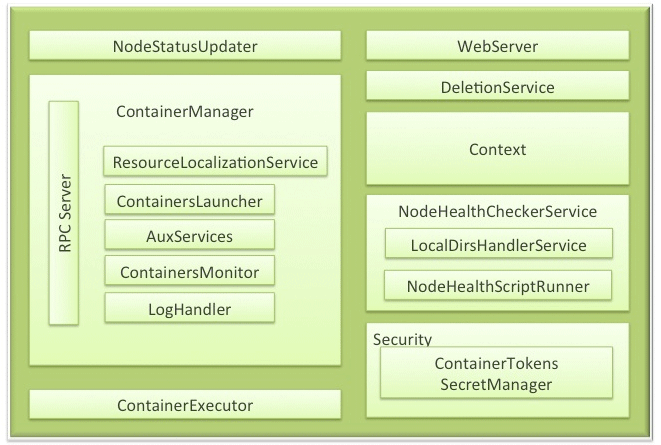
\includegraphics[scale=0.4]{./figures/yarn_NM}
    \label{fig:yarn_NM}
  \end{figure}
\end{frame}

\begin{frame}
\frametitle{YARN Node Manager: Operations}
\begin{itemize}
  \item {\bf Manages communications with the RM}
  \begin{itemize}
    \item Registers, monitors and communicates node resources
    \item Sends heartbeats and container status
  \end{itemize}

\vspace{20pt}

  \item {\bf Manages processes in containers}
  \begin{itemize}
    \item Launches AMs on request from the RM
    \item Launches application processes on request from the AMs
    \item Monitors resource usage
    \item Kills processes and containers
  \end{itemize}

\vspace{20pt}

  \item {\bf Provides logging services}
  \begin{itemize}
    \item Log aggregation and roll over to HDFS
  \end{itemize}
\end{itemize}
\end{frame}

\begin{frame}
\frametitle{YARN Resource Request}
\begin{block}{Resource Request}
  \begin{itemize}
    \item {\bf Resource name:} hostname, rackname, *
    \item {\bf Priority:} within the same application, not across apps
    \item {\bf Resource requirements:} memory, CPU, and more to come...
    \item {\bf Number of containers}
  \end{itemize}
\end{block}
\begin{figure}[h]
  \centering
  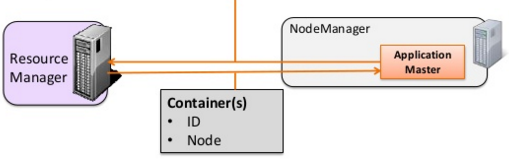
\includegraphics[scale=0.4]{./figures/yarn_resource}
  \label{fig:yarn_resource}
\end{figure}
\end{frame}

\begin{frame}
\frametitle{YARN Containers}
\begin{block}{Container Launch Context}
  \begin{itemize}
    \item {\bf Container ID}
    \item {\bf Commands to start application task(s)}
    \item {\bf Environment configuration}
    \item {\bf Local resources:} application/task binary, HDFS files
  \end{itemize}
\end{block}
\end{frame}

\begin{frame}
\frametitle{YARN Fault Tolerance}
\begin{itemize}
  \item {\bf Container failure}
  \begin{itemize}
    \item AM re-attempts containers that complete with exceptions or fail
    \item Applications with too many failed containers are considered failed
  \end{itemize}

\vspace{30pt}

  \item {\bf AM failure}
  \begin{itemize}
    \item If application or AM fail, the RM will re-attempt the whole application
    \item Optional strategy: job recovery
    \begin{itemize}
      \item If fals, all containers are re-scheduled
      \item If true, uses state to find which containers succeeded and which failed, to re-schedule only failed ones
    \end{itemize}
  \end{itemize}
\end{itemize}
\end{frame}

\begin{frame}
\frametitle{YARN Fault Tolerance}
\begin{itemize}
  \item {\bf NM failure}
  \begin{itemize}
    \item If NM stops sending heartbeats, RM removes it from active node list
    \item Containers on the failed node are re-scheduled
    \item AM on the failed node are re-submitted completely
  \end{itemize}
  
\vspace{30pt}

  \item {\bf RM failure}
  \begin{itemize}
    \item No application can be run if RM is down
    \item Can work in active-passive mode (just like the NN of HDFS)
  \end{itemize}
\end{itemize}
\end{frame}

\begin{frame}
\frametitle{YARN Shuffle Service}
\begin{figure}[h]
  \centering
  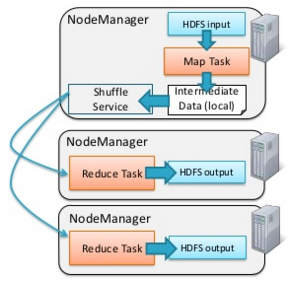
\includegraphics[scale=0.4]{./figures/yarn_shuffle}
  \label{fig:yarn_shuffle}
\end{figure}
\begin{itemize}
  \item {\bf The Shuffle mechanism is now an auxiliary service}
  \begin{itemize}
    \item Runs in the NM JVM as a persistent service
  \end{itemize}
\end{itemize}
\end{frame}

%%%%%%%%%%%%%%%%%%%%%%%%%%%%%%%%%%%%%%%%%%%%%%%%%%%%%%%%%%%%%%%%%%%%%%%%%%%%%%%
\subsection{YARN Application Example}
%%%%%%%%%%%%%%%%%%%%%%%%%%%%%%%%%%%%%%%%%%%%%%%%%%%%%%%%%%%%%%%%%%%%%%%%%%%%%%%
\begin{frame}
 \begin{colorblock}{blue}{lightblue}{ }
    \Large \textbf{YARN Application Example}
  \end{colorblock}
\end{frame}

\begin{frame}
\frametitle{YARN WordCount execution}
\begin{figure}[h]
  \centering
  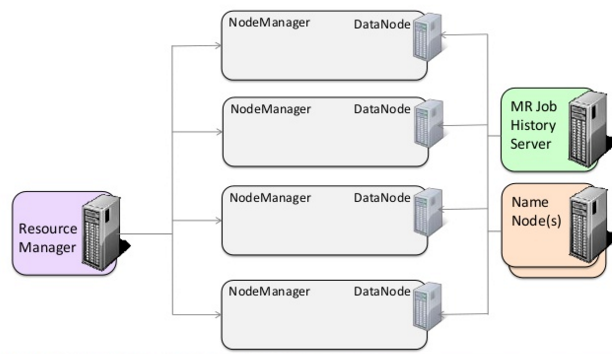
\includegraphics[scale=0.4]{./figures/yarn_wc1}
  \label{fig:yarn_wc1}
\end{figure}
\end{frame}

\begin{frame}
\frametitle{YARN WordCount execution}
\begin{figure}[h]
  \centering
  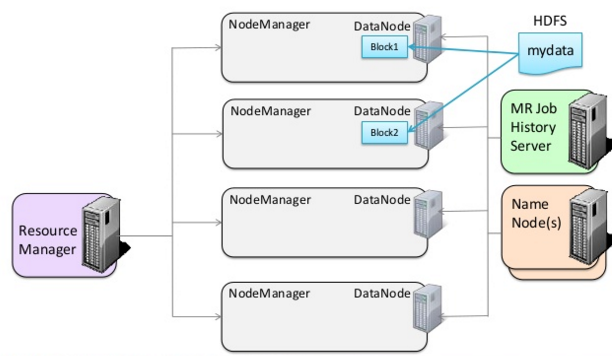
\includegraphics[scale=0.4]{./figures/yarn_wc2}
  \label{fig:yarn_wc2}
\end{figure}
\end{frame}

\begin{frame}
\frametitle{YARN WordCount execution}
\begin{figure}[h]
  \centering
  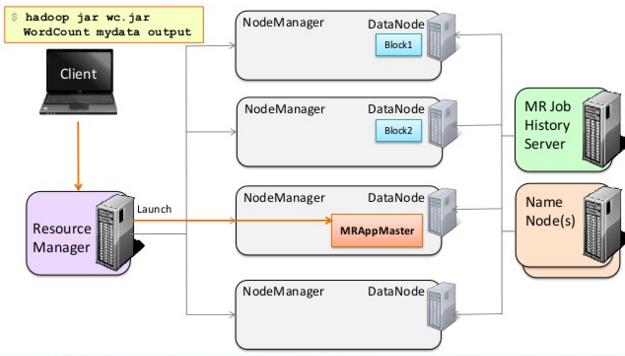
\includegraphics[scale=0.4]{./figures/yarn_wc3}
  \label{fig:yarn_wc3}
\end{figure}
\end{frame}

\begin{frame}
\frametitle{YARN WordCount execution}
\begin{figure}[h]
  \centering
  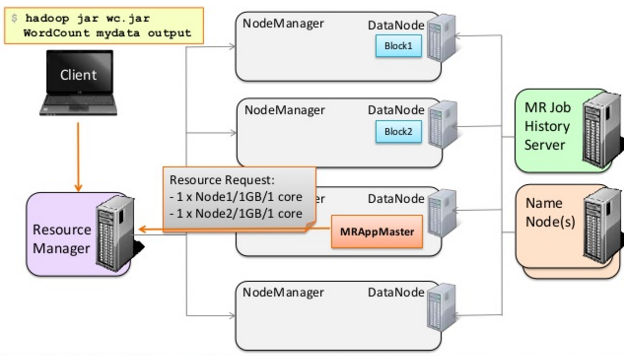
\includegraphics[scale=0.4]{./figures/yarn_wc4}
  \label{fig:yarn_wc4}
\end{figure}
\end{frame}

\begin{frame}
\frametitle{YARN WordCount execution}
\begin{figure}[h]
  \centering
  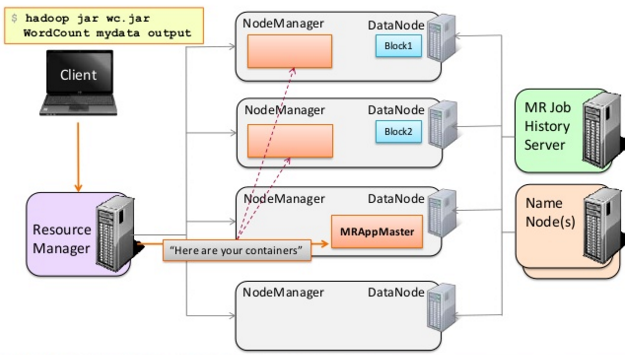
\includegraphics[scale=0.4]{./figures/yarn_wc5}
  \label{fig:yarn_wc5}
\end{figure}
\end{frame}

\begin{frame}
\frametitle{YARN WordCount execution}
\begin{figure}[h]
  \centering
  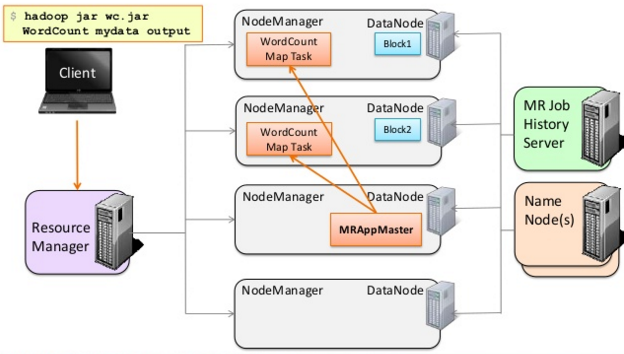
\includegraphics[scale=0.4]{./figures/yarn_wc6}
  \label{fig:yarn_wc6}
\end{figure}
\end{frame}

\begin{frame}
\frametitle{YARN WordCount execution}
\begin{figure}[h]
  \centering
  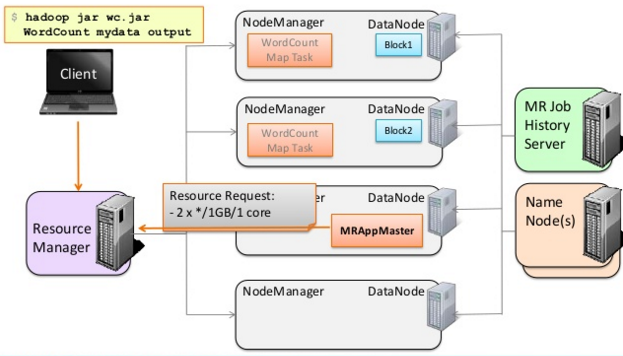
\includegraphics[scale=0.4]{./figures/yarn_wc7}
  \label{fig:yarn_wc7}
\end{figure}
\end{frame}

\begin{frame}
\frametitle{YARN WordCount execution}
\begin{figure}[h]
  \centering
  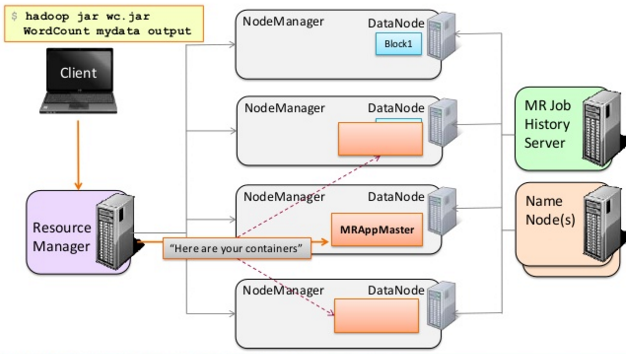
\includegraphics[scale=0.4]{./figures/yarn_wc8}
  \label{fig:yarn_wc8}
\end{figure}
\end{frame}

\begin{frame}
\frametitle{YARN WordCount execution}
\begin{figure}[h]
  \centering
  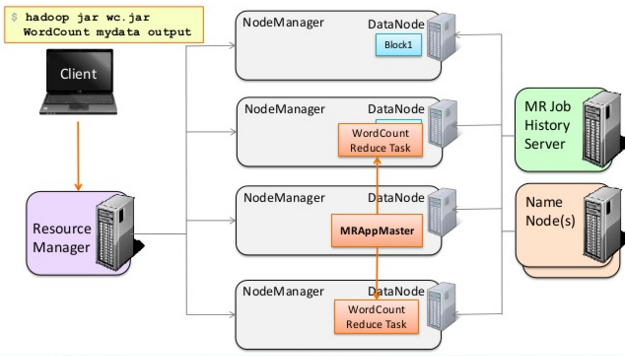
\includegraphics[scale=0.4]{./figures/yarn_wc9}
  \label{fig:yarn_wc9}
\end{figure}
\end{frame}

\begin{frame}
\frametitle{YARN WordCount execution}
\begin{figure}[h]
  \centering
  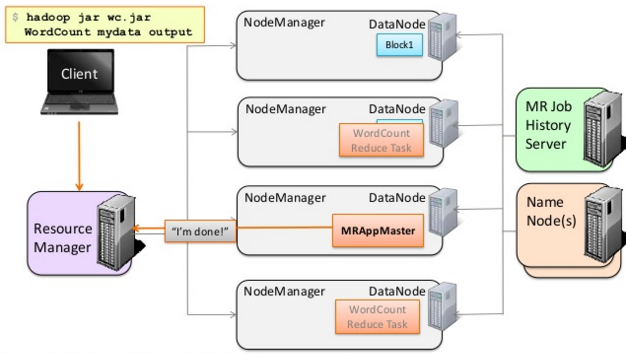
\includegraphics[scale=0.4]{./figures/yarn_wc10}
  \label{fig:yarn_wc10}
\end{figure}
\end{frame}
